\documentclass[amsmath,amssymb,notitlepage,12pt]{revtex4}
%\documentclass[12pt]{article}
\usepackage[toc,page]{appendix}
\usepackage{graphicx}
\usepackage{bm}% bold math
\usepackage{multirow}
\usepackage{booktabs}
\usepackage{verbatim}
\usepackage{hyperref}
\usepackage{enumitem}
\hypersetup{pdftex,colorlinks=true,allcolors=blue}
\usepackage{hypcap}
\usepackage[small,compact]{titlesec}
\setlist[enumerate]{itemsep=0mm}
%\addtolength{\textwidth}{1.3cm}
%\addtolength{\hoffset}{-0.7cm}
%\addtolength{\textheight}{2.8cm}
%\addtolength{\voffset}{-0.4cm}
\begin{document}
\title{CLAS12 M{\o}ller Operations Manual - v1.4}
\date{\today}
\author{N. Baltzell, S. Stepanyan}
\begin{abstract}
\end{abstract}

\maketitle
%\tableofcontents
%\newpage

\section{Introduction}
The CLAS12 M{\o}ller system measures the polarization of the electron beam delivered to Hall B, and this document details its operating procedures.  The user interface for shift workers is shown in Fig.~\ref{fig:unconfig} and provides direct access to all controls and feedback that the normal operator should need, and its operating procedures are described in Section~\ref{sec:user}.%  Expert operations are described in Appendix~\ref{sec:expert}.

{\em \large Note, M{\o}ller runs must be performed with acceptable beam delivered to the {\bf tagger dump/yoke};  consult the beamline manual for general procedures on establishing beam if necessary.}

\begin{figure}[htbp]\centering
    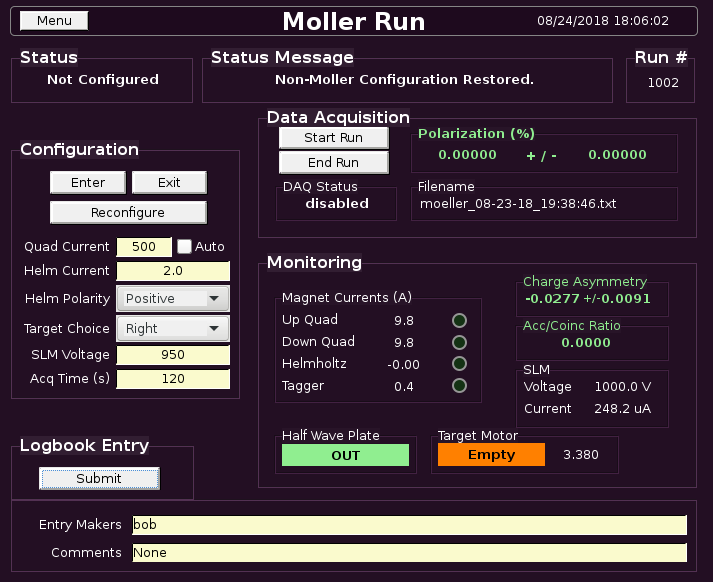
\includegraphics[width=11cm]{pics/unconfig}
    \caption{The user interface for shift workers for operating a M{\o}ller run is divided into {\em Status}, {\em Configuration}, {\em Data Acquisition}, {\em Monitoring}, and {\em Logbook} sections.  In this screenshot, the M{\o}ller system is not configured, according to the {\em Status} section, i.e. the setup is for non-M{\o}ller beam delivery.\label{fig:unconfig}}
\end{figure}

\newpage

\section{Hardware Settings}
The standard hardware settings for a M{\o}ller run are shown in Table~\ref{tab:pars}.  These are displayed in the {\em Configuration} section of Figure~\ref{fig:unconfig} and will be used to automatically configure all hardware during the procedure in Section \ref{sec:user}.  It is the responsibility of the operator to ensure that the settings in the {\em Configuration} section are the desired ones before entering the M{\o}ller setup.
\begin{table}[htbp]\centering
    \begin{tabular}{ll}\toprule[1.5pt]
        SLM Voltage & 1400 V \\
        Collimator Position & Blank \\
        Target Position & Left \\
        Helmholtz Current & $\pm$3.5 A \\
        \cmidrule[0.5pt]{1-2}
        \multicolumn{2}{c}{Quadrupole Current} \\
        5-pass / 10.7 GeV & 3145 A\\
        3-pass / 6.4 GeV & 1350 A\\
        \bottomrule[1.5pt]
    \end{tabular}
    \caption{Standard hardware parameter values for the M{\o}ller setup.  Live values are shown in the {\em Monitoring} section in Figure~\ref{fig:unconfig}.\label{tab:pars}}
\end{table}

\section{Quality Requirements}\label{sec:quality}
The requirements to be maintained during a M{\o}ller run, and the resulting desired error on the polarization measurement are shown in Table~\ref{tab:reqs}.  It is the responsibility of the operator to monitor these quantities to ensure a successful polarization measurement.
\begin{table}[htbp]\centering
    \begin{tabular}{ll}\toprule[1.5pt]
        2C21 BPM Current & $\sim$4 nA\\
        Beam Charge Asymmetry & $<0.2\%$ (typical $\sim 0.1\%$)\\
        Accidental/Coincidence Ratio & $<0.1$ (typical $\sim 0.05$)\\
        Final Beam Polarization Error & $<1.5\%$ (absolute)\\
        \bottomrule[1.5pt]
    \end{tabular}
    \caption{Standard quality conditions required for a M{\o}ller run.  Live values are shown in the {\em Monitoring} and {\em Data Acquisition} sections in Figure~\ref{fig:unconfig}.  Note, beam polarization error depends on statistics and should gradually decrease during the run.\label{tab:reqs}}
\end{table}

\newpage

\section{Standard Procedures}\label{sec:user}
Before starting the M{\o}ller procedure, confirm that Hall B orbit locks are off and our Halo and BOM FSD are masked.
\subsection{Procedure Summary}
The procedure for the operator with the interface in Figure~\ref{fig:unconfig} can be summarized in the following steps, and more details are shown on the next section.
\begin{enumerate}
\vspace{-4mm}\item {\bf Request No Beam:}  ask MCC to take beam away for a configuration change
\vspace{-4mm}\item {\bf Configure:}  ensure the Configuration section is set as desired
\vspace{-4mm}\item {\bf Enter:} click {\em Enter} in the Configuration section and wait for success status
\vspace{-4mm}\item {\bf Request 4 nA:} ask MCC to resume beam delivery at 4 nA for M{\o}ller runs
\vspace{-4mm}\item {\bf Start Run:} click {\em Start Run} in the DAQ section
\vspace{-4mm}\item {\bf Monitor:} monitor the critical parameters
\vspace{-4mm}\item {\bf End Run:} click {\em End Run} in the DAQ section
\vspace{-4mm}\item {\bf Log Entry:} click {\em Submit} in the Logbook Entry section 
\vspace{-4mm}\item {\bf Request No Beam:} ask MCC to take beam away for a configuration change
\vspace{-4mm}\item {\bf Reconfigure:} (Optional)
\vspace{-4mm}\item {\bf Exit:} click {\em Exit} in the Configuration section and wait for success status
\end{enumerate}

\subsection{Procedure Details}
\begin{enumerate}
    \item {\bf Request No Beam:}  ask MCC to take beam away while you configure the M{\o}ller system
    \item {\bf Configure:}  ensure the Configuration section of Fig.~\ref{fig:unconfig} is set as desired
        \subitem
        See Table~\ref{tab:pars} for standard values.  Contact the Run Coordinator if uncertain.
        %If the {\em Auto} option is selected for the quadrupoles, their current will be chosen based on standard settings for the current beam energy.
        %{\em Note, it is critical that some of these settings are held fixed while a run is ongoing, and those cannot be changed during a run from this interface.  See below regarding reconfiguring.}
\item {\bf Enter:} click {\em Enter} in the Configuration section and wait for success status
    \subitem This will configure the system for a M{\o}ller run by initiating a sequence of actions and provide corresponding feedback in the status portion of the screen.  This includes turning off all appropriate detectors' high voltage, inserting the blank collimator, energizing the quadrupoles and Helmholtz magnets, and inserting the M{\o}ller target.  Success will result in ``Moller Configuration Ready'' in the status message.
\item {\bf Request 4 nA:} \label{step:beam} ask MCC to resume beam delivery at 4 nA for M{\o}ller runs
\item {\bf Start:} \label{step:start} once beam is stable, click {\em Start Run} in the DAQ section
    \subitem This will initiate a new M{\o}ller run, including zeroing any accumulated data, opening a new data file, incrementing the run number, and starting data acquisition.
\item {\bf Monitor:} monitor the critical quality parameters
    \subitem This is left to the operator, described in Table~\ref{tab:reqs}, with possible actions in Section~\ref{sec:knobs}.  Of particular importance are beam charge asymmetry below 0.2\% and accidental ratio of less than 0.1, although ideally about half that.  {\em If you cannot achieve the quality requirements, contact the Run Coordinator.}
\item {\bf End:} click {\em End Run} in the DAQ section
    \subitem At this point you should have achieved the desired polarization error of $1.5\%$ (see Table~\ref{tab:reqs}), or just need to stop the current run and start a new one (in which case, go to Step \#\ref{step:start}).
\item {\bf Log Entry}: click {\em Submit} in the Logbook Entry section if the run was successful. 
    \subitem This will submit a standardized, searchable log entry to HBLOG with a table summarizing the results and an attached data file, and requires filling the Entry Makers and Comments fields.  {\em Note, if you want to log any screenshots associated with this M{\o}ller run, then you should navigate to this log entry and upload them as comments}.
    \subitem Note, at this point you can start another run with the same configuration by going to Step \#\ref{step:start}.
\item {\bf Request No Beam:} ask MCC to take beam away before changing the M{\o}ller configuration
\item {\bf Reconfigure:}  (Optional)  At this point you may reconfigure the system (e.g. change the Helmholtz polarity or switch to a different target, and then click {\em Reconfigure}, or just ask for a change in the Half-Wave Plate) and then start another run (go to Step \#\ref{step:beam}).
\item {\bf Exit}: click {\em Exit} in the Configuration section and wait for success status
    \subitem  This will restore the non-M{\o}ller configuration by turning off the quadrupoles and Helmholtz and retracting the M{\o}ller target.  {\em Note, this will not restore any detector high voltage (except the SLM) nor move the collimator}. 
\end{enumerate}

\newpage
\section{Quality Requirements}\label{sec:knobs}

If quality requirements are not satisfied (accidental rate and beam charge asymmetry), first check whether our hardware settings are as expected by comparing to the parameters earlier in this document and also to recent satisfactory M{\o}ller runs in the logbook.  The following subsections contain information on the quality measurements and the main parameters that can affect them.  Consult with the Run Coordinator and/or beamline expert for advice on tuning these parameters, and compare their values with previous M{\o}ller runs.

\subsection{Run Duration}
At 10 GeV, with our 2018 hardware configuration, the normal run duration to achieve 1.5\% absolute error on the polarization is about 30 minutes of continuous beam.  Interruptions to beam delivery, e.g. trips, will of course increase the necessary run time.  Much longer than normal run duration to achieve 1.5\% can be indicative of excessive accidentals or beam charge asymmetry.

\subsection{Beam Charge Asymmetry}
Beam charge asymmetry is measured by a Synchrotron Light Monitor fed to a Struck scaler latching on the heliticy signals.  The SLM is located a few meters upstream of, and {\em completely independent of}, the rest or our M{\o}ller system.  Beam Charge asymmetry is affected primarily by beam characteristics from the injector and accelerator.  There can be some effect from quality of the SLM performance, e.g. if voltage is far too high and the SLM is saturated, but this should generally never be the case for the normal operator.

Note that beam charge asymmetry updates with the same period as our Moller acquisition time, i.e. if the acquisition time is set at 60 seconds, beam charge asymmetry will only update once per minute.%  It can be important not to gauge the quality based on only one or two readings, but to assess based on multiple readings with stable beam.%  To facilitate this, one can open a strip chart to monitor beam charge asymmetry over time, or increase the acquisition time for a higher statistics reading during stable beam.

If the beam charge asymmetry is too high, the parameters that can be considered are:
\begin{itemize}
\vspace{-4mm}\item Beam position (BPM and harp scans)
\vspace{-4mm}\item Beam profile (harp scans)
\vspace{-4mm}\item Injector slit setting
\vspace{-4mm}\item Injector attenuator settings
\end{itemize}

\subsection{Accidentals}
The accidental-coincidence ratio is measured by M{\o}ller Left/Right PMTs, downstream of the target and quadrupoles, and is independent of the helicity signals.  Excessive accidentals can be caused by beam quality issues, e.g. bleedthrough from other halls, or non-optimal settings of our M{\o}ller system.  Parameters that can be considered for adjustment include the same beam quality parameters in the previous section, and with the addition of our M{\o}ller configuration, e.g. Left/Right PMT voltages, malfunctioning quadrupoles, or very miscalibrated target position.

%\newpage
%\section{Status Values}
%Describe the possible values of the status variable in the top left of the screen.

%\begin{appendices}
%%\section{Expert Procedures}\label{sec:expert}
%%{\bf\em Note, this section may be out of date and should be ignore by shift operators.}

\subsubsection{Before start}

\begin{itemize}
\item Reasonable quality beam must be already present for Hall-B
\item Beam has to be terminated on the tagger-yoke dump
\item CLAS12 is OFF, especially sensitive detectors: HV on \textbf{Drift Chambers} and \textbf{SVT/MVT}
\end{itemize}
%\item Harps are in the retracted position.
%\item Beam current should be set  to $\le 10$ nA 

%The optimal beam current is a function of beam energy. More specific information may be available on the white board in the counting house or in the run period specific documentation on the run wiki. Regardless of what currents are specified on the White board or in this document, the ratio $Left\otimes Right$ accidentals to the true coincidence rate should be kept below 5\%. It may be necessary to adjust the HV on the Left and Right PMT's to achieve a low accidental rate, while maintaining a reasonable true coincidence rate.

\subsubsection{Setup }

\begin{enumerate}
\item Notify MCC that you are about to do M{\o}ller run and \textbf{request
to take the beam to the tagger yoke beam dump} (they will need to take the beam
away and energize the tagger magnet), MCC will ask to change BTA setting to ``photon" 
\item Ask MCC to turn orbit locks off, and mask BOM and Halo Counters in FSD 
\item Turning ON the polarimeter is done from EPICS GUIs (for now multiple control GUIs in expert mode are used). \\
{\bf NOTE: BEAM SHOULD BE OFF DURING the SETUP of M{\o}LLER POLARIMETER}\\
M{\o}ller setup GUIs can be launched from the \textbf{Moeller} tab on the \emph{"clascss"} GUI. 
%\latex{\ref{fig:moller_epics}} on page\pageref{{fig:moller_epics} } shows the
%M{\o}ller system GUI before the hardware has been set up. 

\begin{enumerate}
\item the "Moeller Asym - All" GUI, see Fig.\ref{fig:mainmoller} contains all the helicity gated scalers, charge asymmetry, and the beam polarization\footnote{The polarization and charge asymmetry have GUIs their own, but for now this main GUI will be used.}. It has several controls for the measurement and monitoring: 
\begin{description}
\item[Buttons "Start", "Reset" and "Stop"] will start and stop acquisition of data or reset acquisition (clear scaler buffers). 
\item[The acquisition time] controls update frequency of scalers, measured polarization value, and the charge asymmetry value. It is recommended to have M{\o}ller polarimeter acquisition time $>60$ seconds when taking the measurements. For practical reasons, at the start when charge asymmetry will need tuning (see below) time for the scaler update can be set to $\sim 10$ seconds. The time can be set either by typing a value in the box or moving the slider. 
\item[The "Attenuator Controls"] are to control beam charge asymmetry. By changing voltage on intensity attenuators (IA) one can equalizes intensity across helicity states. It is recommended to use "Global Offset" that will change voltage on all four IAs at the same amount. Desire charge asymmetry is $<0.1\%$ based on SLM. 
\end{description}

%Make sure that the integration time for the asymmetry scalers is set to 5 on the \emph{``asym''} GUI under \emph{``Beamline''}. If it is not, use the slider to set it to 5 (if the slider wont move, check ``IOC ACCESS'' on \emph``clascss'' GUI on clonsl) 

\begin{figure}
\begin{center}
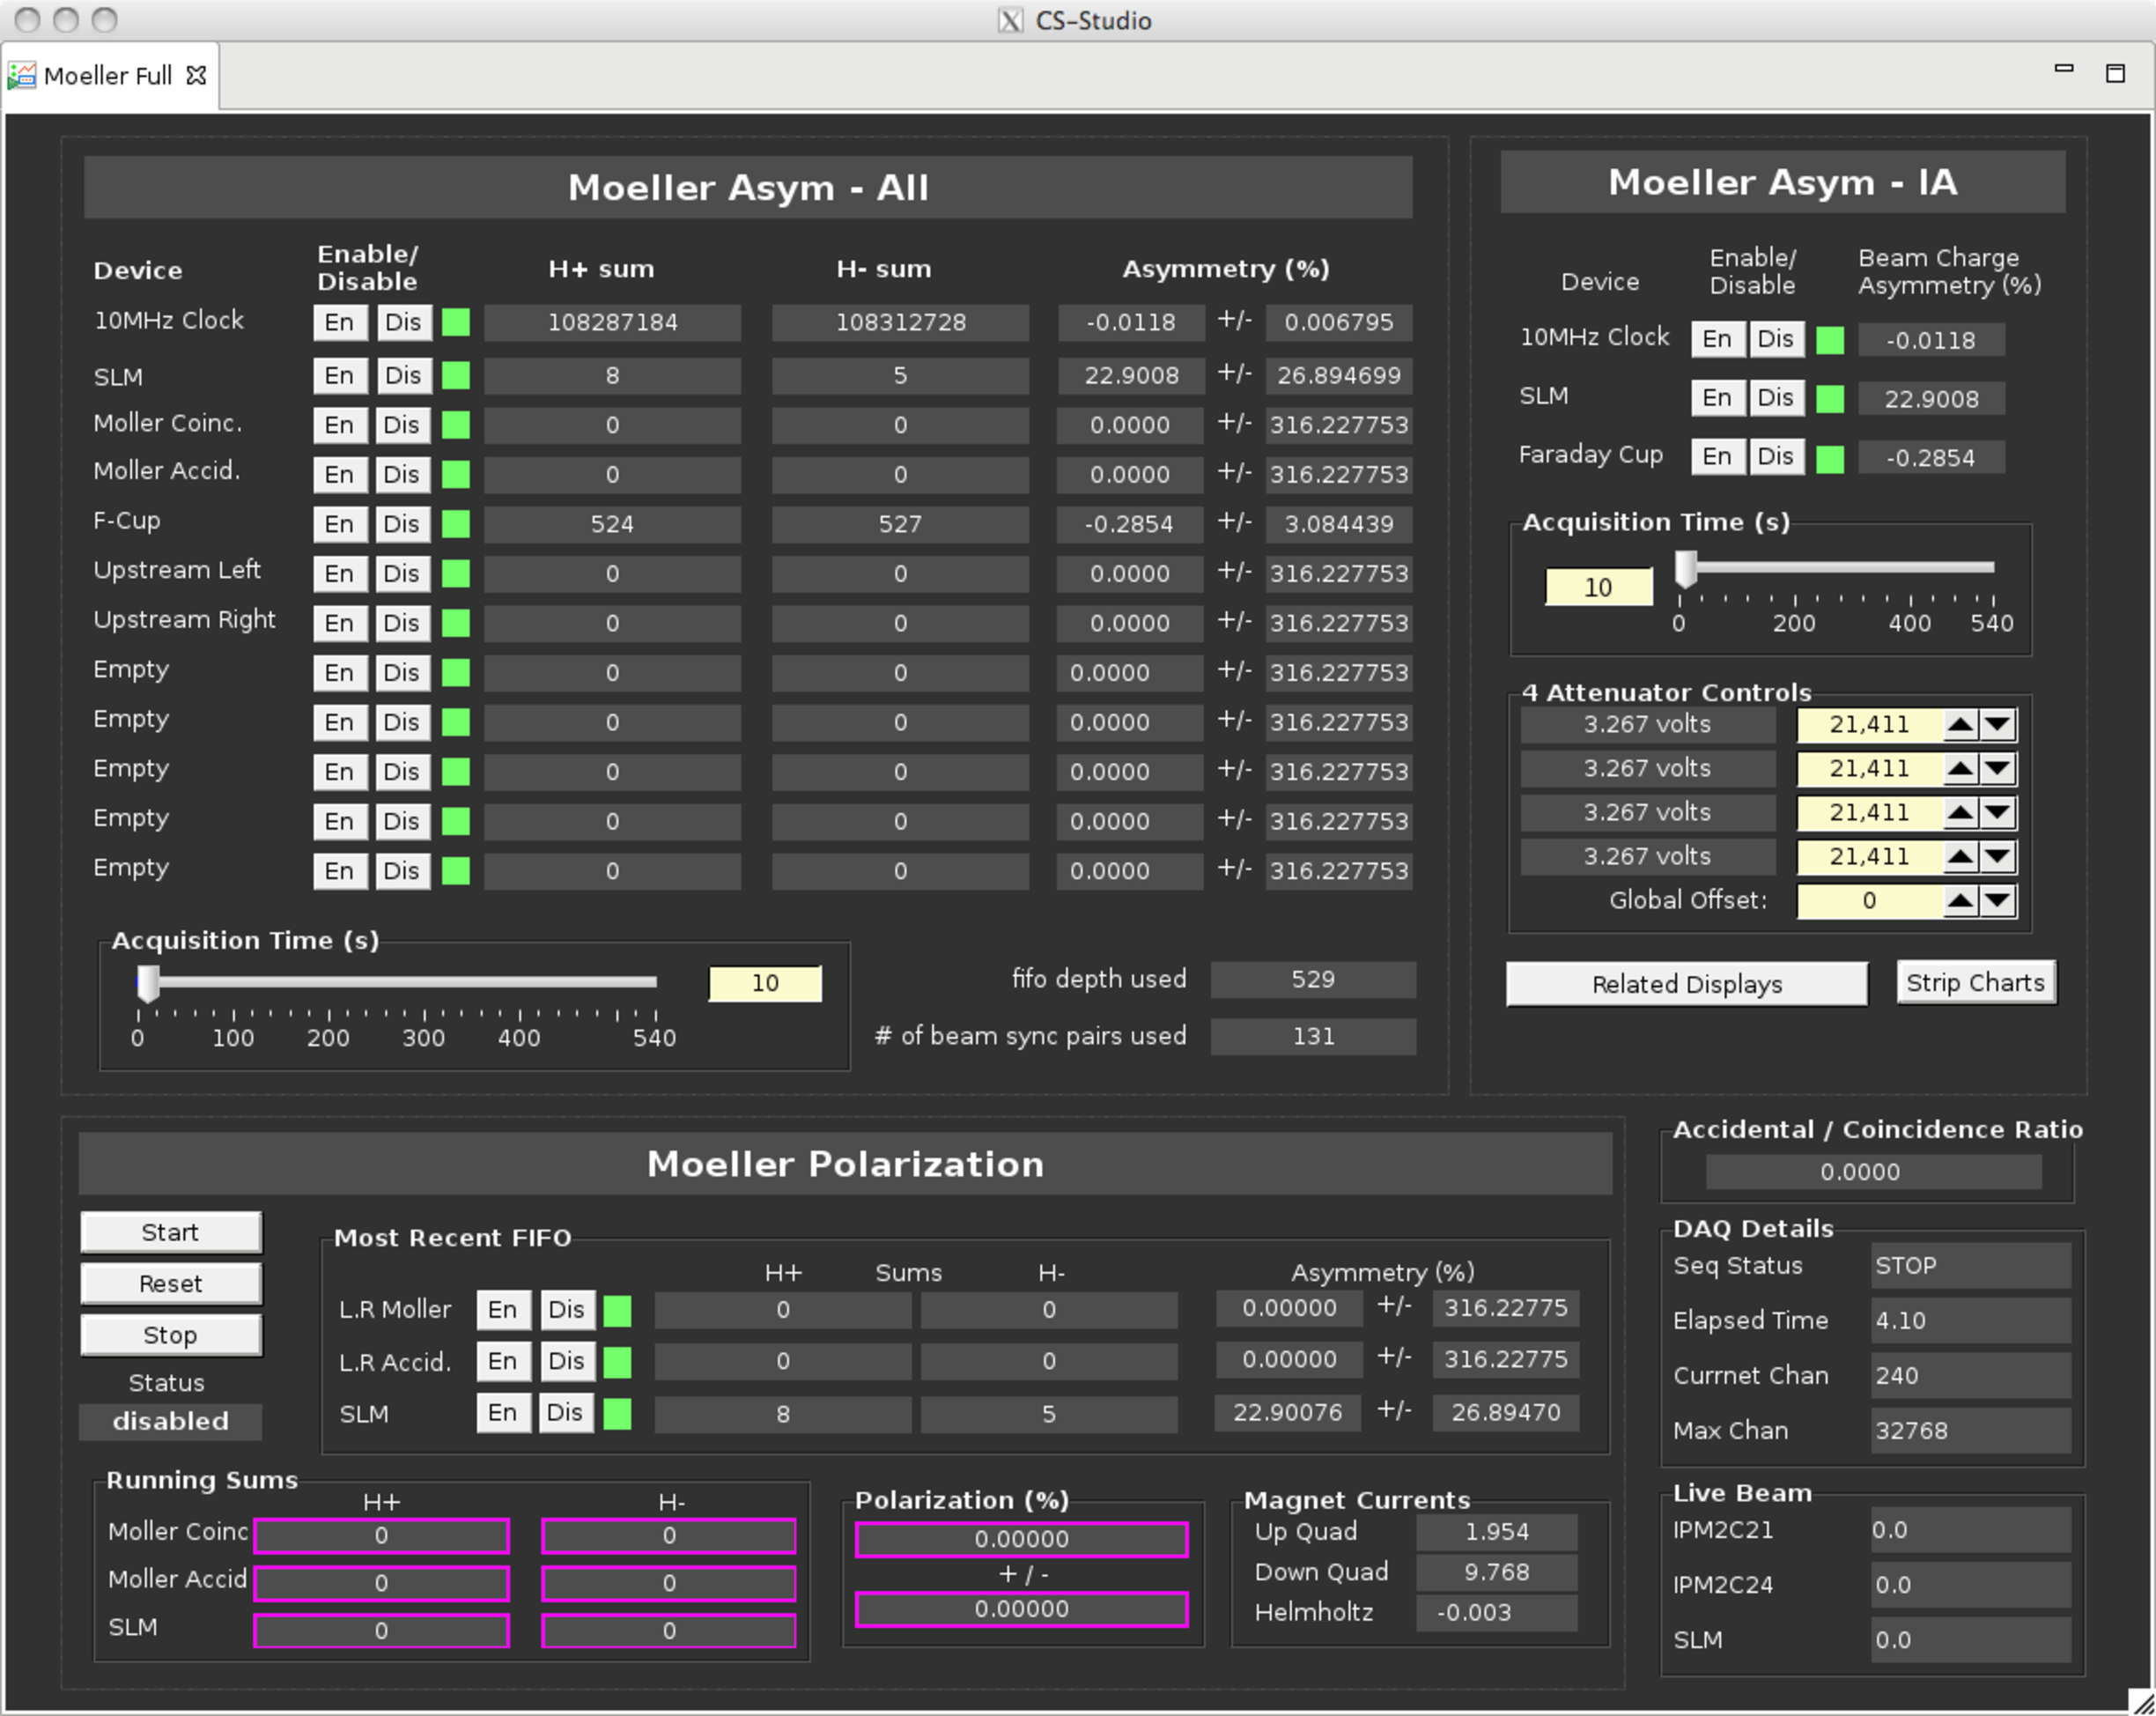
\includegraphics[width=0.8\textwidth]{pics/moller_asym_all.pdf}
\caption{The main M{\o}ller Epics expert GUI.}
\label{fig:mainmoller}
\end{center}
\end{figure}

\item The control for M{\o}ller quadrupole power supplies are provided in "Moeller Quadrupoles" GUI, see Fig.\ref{fig:moller_quad}. Power supplies will be turned ON and in remote before hall closing. From GUI one should first turn them on by pushing the "PS ON" buttons, then set the desire value for currents in "Current Setpoint" window. For $10.7$ GeV the suggested value for the quadrupoles is $3050$ A.

\begin{figure}
\begin{center}
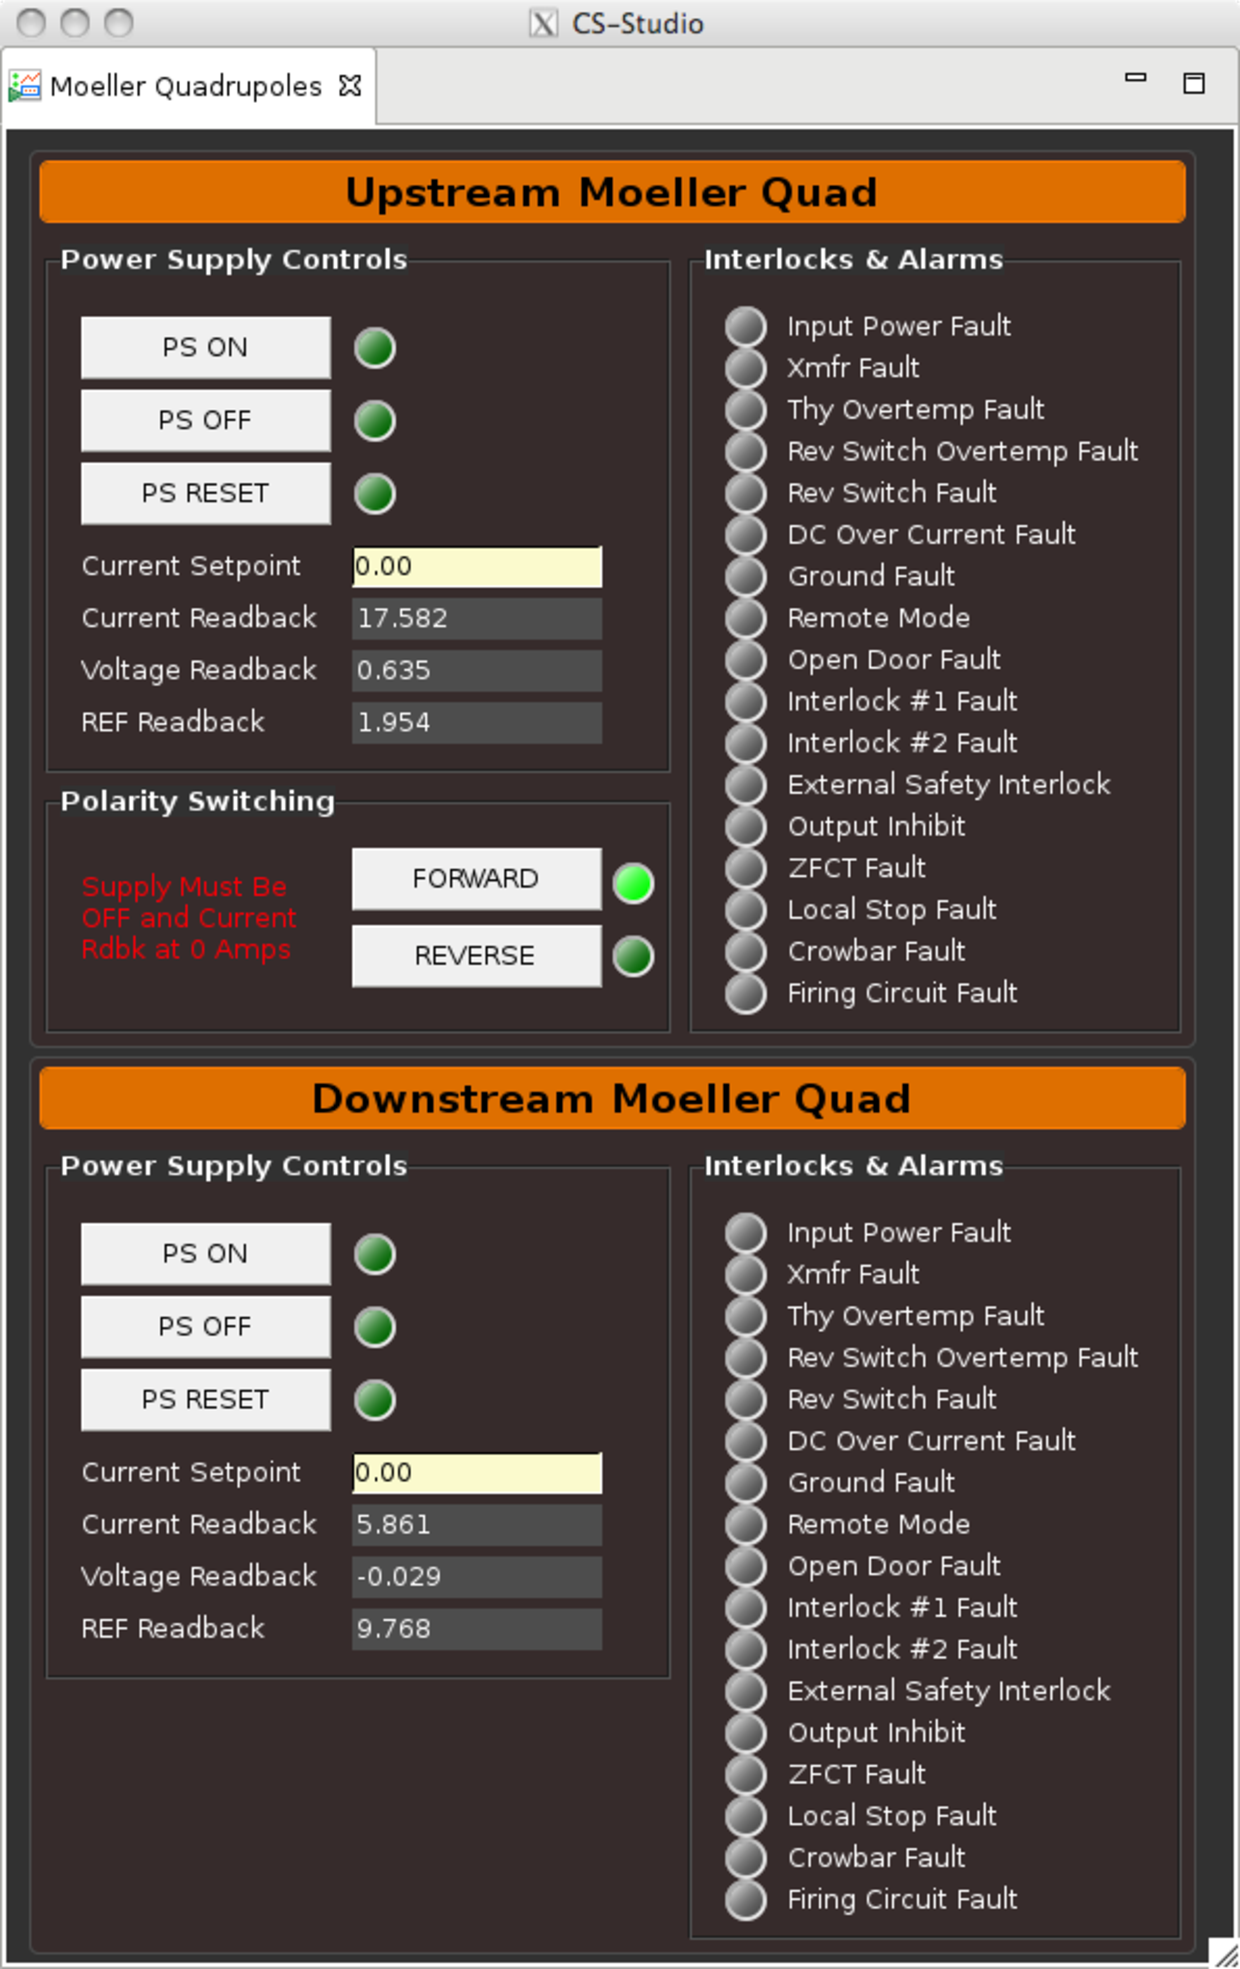
\includegraphics[width=0.75\textwidth]{pics/moller_quad.pdf}
\caption{Control GUI for the M{\o}ller quadrupole power supplies.}
\label{fig:moller_quad}
\end{center}
\end{figure}


%Click \emph{``Configure M{\o}ller Hardware''} button, near the top of the GUI, Figure \ref{fig:moller_epics_setup}. This will start the following sequence of events:

%\begin{enumerate}
%\item SC HV Mainframes will be turned off.
%\item EC HV Mainframes will be turned off.
%\item Helmholtz Magnet will be energized in the Negative polarity.
%\item M{\o}ller Target will be positioned to the \emph{LEFT} target position.
%\item M{\o}ller Quadrupole magnets will be energized
%\item EPICS DAQ will be started
%\end{enumerate}
%\item Watch the text at the top of the GUI for informational guidance.

\item The target is polarized to its saturation by a longitudinal (along the beam) magnetic field generated using pair of Helmholtz coils. It is expected that the target will be saturated at $\sim 1.8$ A current in the coils. The recommended current for M{\o}ller measurement is $3$ A. A GUI for power supply of Helmholtz coils, "Moeller Helmholtz PS" see Fig.\ref{fig:moller_helm}, has two controls, button "STATE" defines state of the power supply. Typicaly it will be in "STANDBY" state when is not used. To energize coils first from the menu in "STATE" chose PS ON, then in "Current Setpoint", a white window, write the value, either $3$ or $-3$. Beam polarization measurements with both orientations the Helmholtz field is recommended to check systematics.    

\begin{figure}
\begin{center}
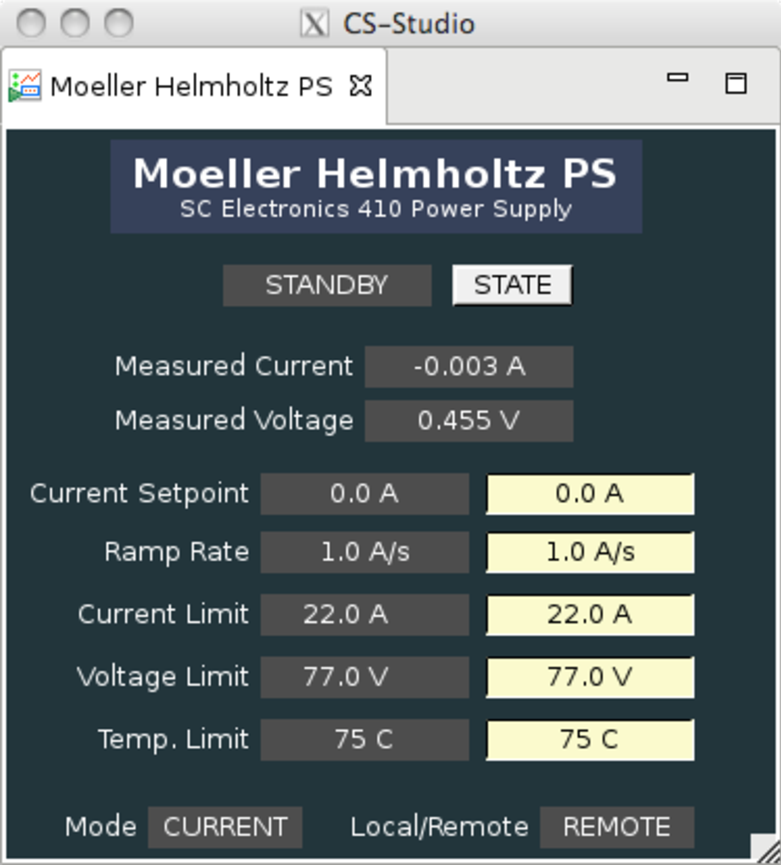
\includegraphics[width=0.65\textwidth]{pics/moller_helmholtz.pdf}
\caption{Control GUI for the M{\o}ller target Helmholtz coils power supply.}
\label{fig:moller_helm}
\end{center}
\end{figure}
%\clearpage

\item a target control GUI, Fig.\ref{fig:moller_target}, allows to position desired target on the beam. Left target is the recommended target for the measurements.

\begin{figure}
\begin{center}
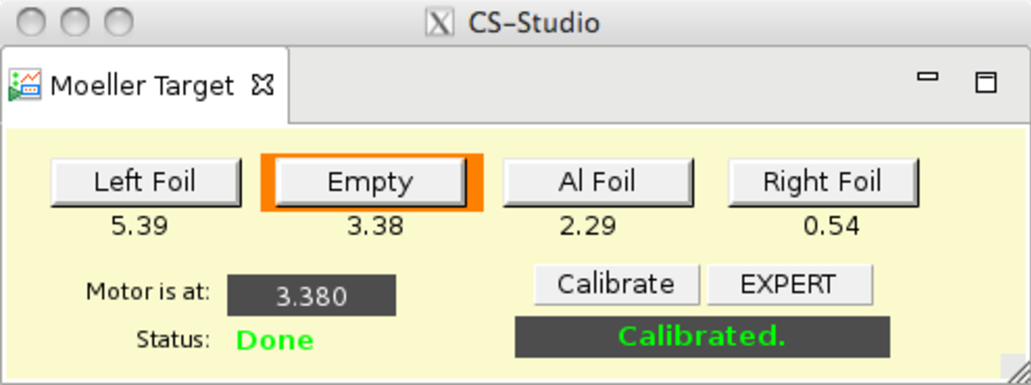
\includegraphics[width=0.65\textwidth]{pics/moller_target.pdf}
\caption{Control GUI for the M{\o}ller target.}
\label{fig:moller_target}
\end{center}
\end{figure}

\end{enumerate}
%
%\clearpage

\item Once the tagger magnet is energized, M{\o}ller setup is UP and ready, request the beam current as specify for the given energy M{\o}ller measurements to be delivered\footnote{The optimal beam current is a function of beam energy.
More specific information may be available on the white board in the
counting house or in the run period specific documentation on the run wiki. Regardless
of what currents are specified on the white board or in this document,
the ratio $Left\otimes Right$ accidentals to the true coincidence
rate should be kept below 5\%. It may be necessary to adjust the
HV on the Left and Right PMT's to achieve a low accidental rate, while
maintaining a reasonable true rate.}, 
as measured by 2C21 nA BPM and/or SLM. Do
not use 2C24A since that BPM is located downstream of the M{\o}ller setup. For $\sim 11$ GeV beam, if beam conditions are normal, as expected, the beam current should be $4$ nA. 

\end{enumerate}

%\clearpage
\subsubsection{Data Taking}
\indent
\begin{itemize}
\item 
To start a new run when DAQ is still running hit the "Reset" button on "Moeller Asym - All" GUI. If run was stoped hit the "Start" then "Reset". 
\item Run is complete when the error on the beam polarization on the GUI is below $\le 1.5\%$ absolute. Typically it takes about $45$ min to $60$ min to get the required accuracy (beam condition dependent). 
\item Make measurements with both positions of the half-wave plate,  "IN" and "OUT" (start the first measurement with whichever position it is, then do the second measurement with the other setting). 
\item If needed perform measurements with both polarity of the Helmholtz coils. 
\item Log every measurement by sending "Moeller Asym - All" GUI to logbook together with main scaler GUI to document beam currents, beam position, and halo counter rates. 
\end{itemize}

\subsubsection{Backing off M{\o}ller setup out\label{moller cblose out}}

When done with the measurements:
\begin{itemize}
\item Do not forget to make a log entry including all details and the GUI! 

%Click the \emph{Backout Moller Hardware} button on the EPICS GUI to restore the hardware back to production running. 

\item Request MCC to take the beam away and \textbf{de-gauss the tagger
magnet if the next step is to send the beam to Faraday cup (usually it is).}

\item Turn off quadrupoles by setting $0$ in "Current Setpoint"s and then when current readback is at $\sim 0$ A push "PS OFF" button

\item Turn off Helmholtz coils by setting $0$ in the current "Current Setpoint" and change "STSTE" to "STANDBY" when "Measured Current" is $\sim 0$

\item Retract the target by pushing "Empty" button on the target GUI

\item Once tagger magnet is degaussed, restore beam to the Faraday Cup.

\item Turn ON CLAS12
\end{itemize}



%\subsubsubsection{Tips}

%\begin{enumerate}
%\item During a M{\o}ller run the upstream PMTs labeled \char`\"{}up\char`\"{} and \char`\"{}down\char`\"{} may get activated. The half life is around 20 Minutes.~ MCC should ignore those PMTs for at least an hour. 
%\item MOLLER QUADS.~ At times the moller quads will not turn on.~ Using the Moller expert screens controls you can try a few things to get them on first try to click the \char`\"{}RESET\char`\"{} and \char`\"{}ON\char`\"{} buttons.~ Then you could try to click the \char`\"{}OFF\char`\"{} and then \char`\"{}ON\char`\"{} buttons.~ The readback value of the current should be close to the entered set value.
%\item Steering:~ Based on the beam tune, the moller quads may substantially deflect the beam.~ A deflection of 5 mm has been observed.~ 
%\item If the Moller PMT's do not come ON, try to reset them using the beamline HV GUI.
%\end{enumerate}


%
%\section{Hardawre and Software}
%Description of the hardware and software involved in the CLAS12 M{\o}ller system.
%\subsubsection{Quadrupoles}
%The quadrupoles use a Dyapower power supply with communications via classc3 hosting a vxWorks EPICS IOC and DVME628 and .
%\subsubsection{Helmholtz}
%The Helmholtz coils use a SCE410 power supply, located on the first level of the space frame in the electronics racks beam-right.  EPICS controls are running on a clonioc linux server in the counting house, communicating with SCE410 via a MOXA serial-ethernet converter in the same rack. 
%\subsubsection{Synchrotron Light Monitor}
%The SLM is located in the upstream beam tunnel near 2c21.  Controls are located on space frame, level 1.  Its high voltage power supply is beam-left in CND's  CAEN SY527 mainframe, while its signal is routed to a Jorger scaler in classc1, beam-right.
%\subsubsection{Target}
%The target controls are running on classc1, with an OMS motor controller, both beam-right on space frame level 1.
%\subsubsection{Helicity Signal}
%The helicity signals are routed through NIM crates and into the Struck scaler in classc6, all on space frame beam-right. 
%\subsubsection{Struck Multi-Channel Scaler}
%The Struck scaler is located in classc6, beam-right.  It counts SLM and Moller PMT, latched on the helicity signals.
%\subsubsection{Sequencing}
%Automated sequencing of controls is via a softioc in the counting house.
%\end{appendices}

\end{document}

